\documentclass[11pt, english]{article}

\usepackage{multicol}
\usepackage{hyperref}
\usepackage[eng]{felipito}
\usepackage{stfloats}
\usepackage{mathpazo}

\usepackage[margin=0.7in, left=0.7in, right=0.7in]{geometry}

\graphicspath{{./Graphics/}}

% Colors
\definecolor{urlcolor}{rgb}{0,.145,.698}
\definecolor{linkcolor}{rgb}{.71,0.21,0.01}
\definecolor{citecolor}{rgb}{.12,.54,.11}


% Document title
\title{\bf Problem Set 5 \\ Statistics, Computation and
Applications\\[-1ex]}
\author{Felipe del Canto}
\date{November, 2021}
    
\hypersetup{
	breaklinks=true,  % so long urls are correctly broken across lines
    colorlinks=true,
    urlcolor=urlcolor,
    linkcolor=linkcolor,
    citecolor=citecolor,
}

\begin{document}
    
\maketitle
   
\begin{multicols}{2}

\section*{Problem 5.1: Flows and Correlations}

For part (a),

For part (b),

For part (c),

\section*{Problem 5.2: Predicting Trajectories}

For part (a),

For part (b),


\section*{Problem 5.3: Gaussian Processes}

For part (a), consider the squared exponential/RBF covariance function
	$$\kappa(x_{i}, x_{j}) = \sigma^{2}\exp\left(-\frac{(x_{i} - x_{j})^{2}}{2\ell^{2}}\right),$$
where $\sigma^2$ is the signal variance and $\ell$ is the lengthscale. If the signal variance is increased, then all things equal, points will have a higher covariance. In other words, the covariance curve (as a function of distance $|x_{i} - x_{j}|$) is higher, the higher $\sigma^{2}$ is. This is shown in \Cref{fig:rbf-sigma}. Moreover, the image shows the decay is similar among all three functions, reaching values close to zero when the distance is close to 3. On the other hand, varying the lengthscale has different effects on the covariance function. As shown in \Cref{fig:rbf-ell}, changing the lengthscale drastically affects the decaying rate of the function. When $\ell$ is small, the decay is faster than when it is larger.

\begin{figure*}
	\caption{Effect of $\sigma^{2}$ and $\ell$ on the RBF covariance function $\kappa(x_{i}, x_{j})$. Panel (a) shows the effect of varying $\sigma^{2}$, when holding $\ell = 1$ constant. In panel (b) it is shown the effect of varying $\ell$, holding $\sigma^{2} = 1$ constant.}
	\label{rbf}
	\begin{subfigure}{0.48\textwidth}
		\centering
		\caption{$\ell = 1$}
		\label{fig:rbf-sigma}
		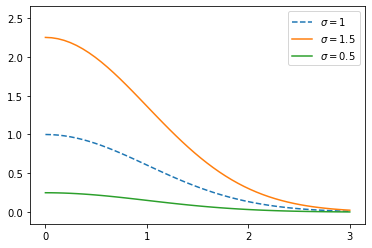
\includegraphics[width=\textwidth]{rbf-sigma}
	\end{subfigure}\hfill
	\begin{subfigure}{0.48\textwidth}
		\centering
		\caption{$\sigma^{2} = 1$}
		\label{fig:rbf-ell}
		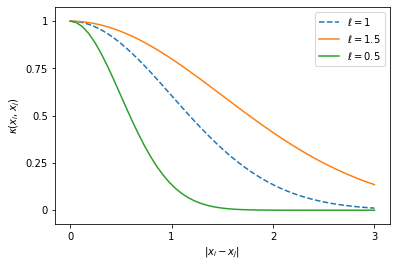
\includegraphics[width=\textwidth]{rbf-ell}
	\end{subfigure}
\end{figure*}


For part (b),

For part (c),




\end{multicols}
\end{document}
